\documentclass{article}[40pt]
\usepackage{ucs}
\usepackage{subcaption}
\usepackage{graphicx}
\usepackage{float}
\usepackage{grffile}
\usepackage[utf8x]{inputenc}
\usepackage[greek,english]{babel}
\usepackage{xspace}
\usepackage{alphabeta}
\usepackage{amssymb}
\usepackage[colorlinks]{hyperref}
\usepackage[fleqn]{mathtools}
\usepackage{adjustbox}
\usepackage{subcaption}
\usepackage{xcolor}
\usepackage{listings}
\hypersetup{
    colorlinks=false,% make the links colored
}

\definecolor{codegreen}{rgb}{0,0.6,0}
\definecolor{codegray}{rgb}{0.5,0.5,0.5}
\definecolor{codepurple}{rgb}{0.58,0,0.82}
\definecolor{backcolour}{rgb}{0.95,0.95,0.92}

\lstdefinestyle{mystyle}{
    backgroundcolor=\color{backcolour},   
    commentstyle=\color{codegreen},
    keywordstyle=\color{magenta},
    numberstyle=\tiny\color{codegray},
    stringstyle=\color{codepurple},
    basicstyle=\ttfamily\footnotesize,
    breakatwhitespace=false,         
    breaklines=true,                 
    captionpos=b,                    
    keepspaces=true,                 
    numbers=left,                    
    numbersep=5pt,                  
    showspaces=false,                
    showstringspaces=false,
    showtabs=false,                  
    tabsize=2
}

\title{ΠΑΝΕΠΙΣΤΗΜΙΟ ΙΩΑΝΝΙΝΩΝ \\ ΤΜΗΜΑ ΜΗΧΑΝΙΚΩΝ Η/Υ  \&  ΠΛΗΡΟΦΟΡΙΚΗΣ \\  ΜΥΕ041 - ΔΙΑΧΕΙΡΙΣΗ ΣΥΝΘΕΤΩΝ ΔΕΔΟΜΕΝΩΝ \\ ΕΡΓΑΣΙΑ 1}
\author{Κίτσιος Κωνσταντίνος 4388 }
\begin{document}
\maketitle
\newpage
\tableofcontents
\newpage
\section{Πηγαίος κώδικας}
Η εκτέλεση του προγράμματος στο τερματικό γίνεται με την εντολή:\\
python3 assignment1.py filename fieldname \\
Όπου filename το όνομα του αρχείου εισόδου και \\
fieldname το όνομα του πεδίου του αρχείου εισόδου (Θα πρέπει να έχει αριθμητικές τιμές).\\
Ο πλήρης κώδικας της εργασίας είναι ο εξής:\\\\

\end{lstlisting}
\newpage
\section{Μέρος 1}
Για το πρώτο μέρος, οι συναρτήσεις που χρησιμοποιούνται για τη δημιουργία των ιστογραμμάτων equi-width \& equi-depth είναι οι equiwidth\_histogram() \& equidepth\_histogram() αντίστοιχα.\\
Η συνάρτηση equiwidth\_histogram(data, bins) υπολογίζει το equi-width histogram ενός πίνακα δεδομένων. Αρχικά υπολογίζει την ελάχιστη και τη μέγιστη τιμή των δεδομένων και καθορίζει το πλάτος του κάθε bin με βάση τον αριθμό των bins που θα χρησιμοποιηθούν. Στη συνέχεια, δημιουργεί έναν πίνακα bin\_ranges και αρχικοποιεί έναν πίνακα hist\_data όπου και θα περιέχει των αριθμό των πλειάδων του κάθε range του bin. Η συνάρτηση διατρέχει τα δεδομένα και αντιστοιχίζει κάθε δεδομένο στο αντίστοιχο bin. Τέλος, επιστρέφει τα δεδομένα του ιστογράμματος και τον πίνακα των ranges του κάθε bin.\\
Η συνάρτηση equidepth\_histogram(data, bins) υπολογίζει το equi-depth histogram ενός πίνακα δεδομένων. Αρχικά ταξινομεί τα δεδομένα και υπολογίζει το μέγεθος του bin και το υπόλοιπο με βάση τον αριθμό των bins που χρησιμοποιούνται. Στη συνέχεια, δημιουργεί έναν πίνακα bin\_ranges και αρχικοποιεί έναν hist\_data όπου και θα περιέχει των αριθμό των πλειάδων του κάθε range του bin. Η συνάρτηση διατρέχει τα bins και αντιστοιχίζει κάθε δεδομένο στο αντίστοιχο bin. Τέλος, επιστρέφει τα δεδομένα του ιστογράμματος και τον πίνακα των ranges του κάθε bin.
\section{Μέρος 2}
Στο δεύτερο μέρος υλοποείται επιπλέον η συνάρτηση estimate\_tuples()  για να εκτιμήσουμε πόσες πλειάδες έχει το
αποτέλεσμα μιας ερώτησης επιλογής στο πεδίο Income, η οποία έχει σαν συνθήκη το $α \leq Income < β.$ \\
Η συγκεκριμένη συνάρτηση υπολογίζει το πλήθος των tuples που βρίσκονται σε ένα δοσμένο εύρος [a, b), βασιζόμενη στα δεδομένα του ιστογράμματος και του πίνακα bins\_ranges  που είναι και ορίσματα της συνάρτησης. Αρχικά επαναλαμβάνει τον πίνακα bins\_ranges για να βρει τα αντίστοιχα bins που επικαλύπτονται με το δοσμένο εύρος. Έπειτα, υπολογίζει το ποσοστό του πίνακα που εμπίπτει στο δοσμένο εύρος και το πολλαπλασιάζει με τον αριθμό των tuples σε εκείνον τον πίνακα. Τέλος, επιστρέφει το συνολικό πλήθος των tuples στο δοσμένο εύρος.
\newpage
\subsection{Equi-width vs Equi-depth histogram}
Παρακάτω φαίνονται τα αποτελέσματα των πειραμάτων δοκιμάζοντας έναν μεγάλο αριθμό ερωτήσεων με διάφορα εύρη.\\
\begin{figure}[htpb!]
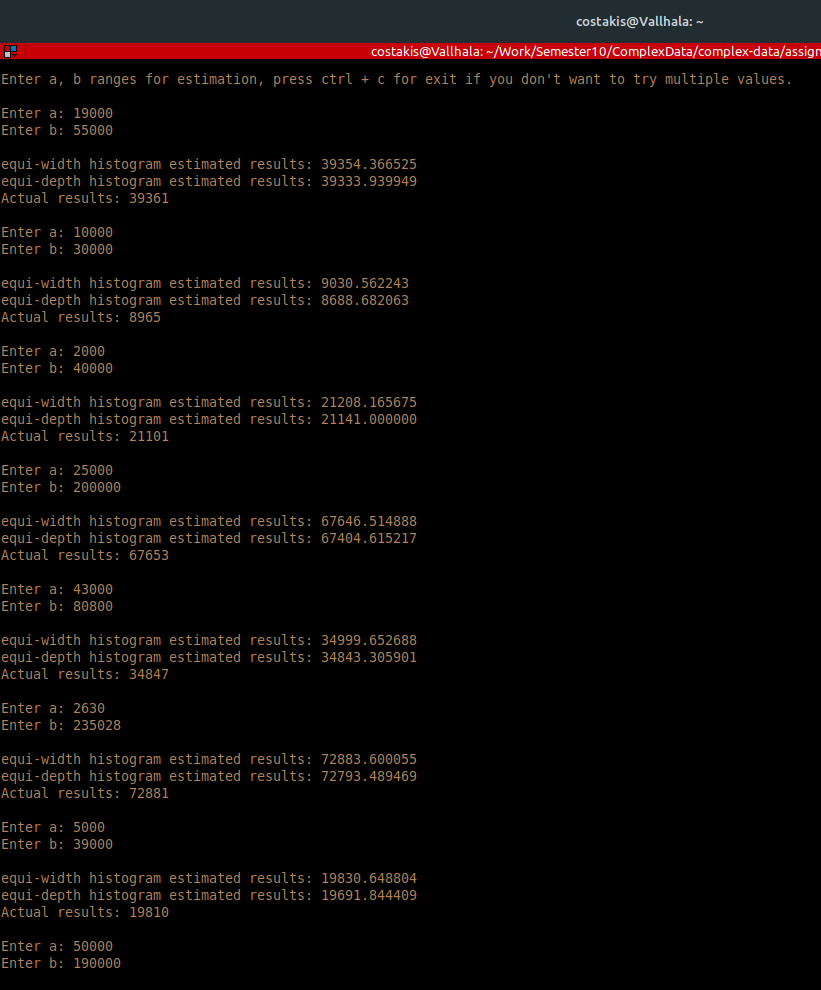
\includegraphics[scale=0.4]{estimations1.png}
\end{figure}
\begin{figure}[htpb!]
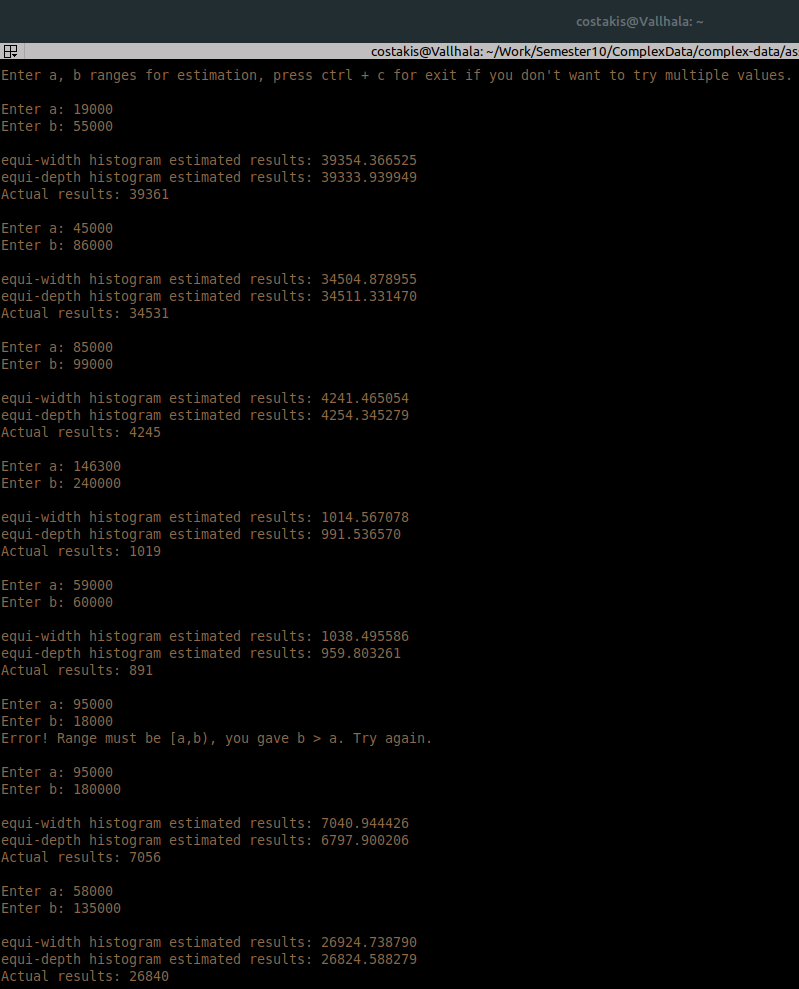
\includegraphics[scale=0.4]{estimations2.png}
\end{figure}
\begin{figure}[htpb!]
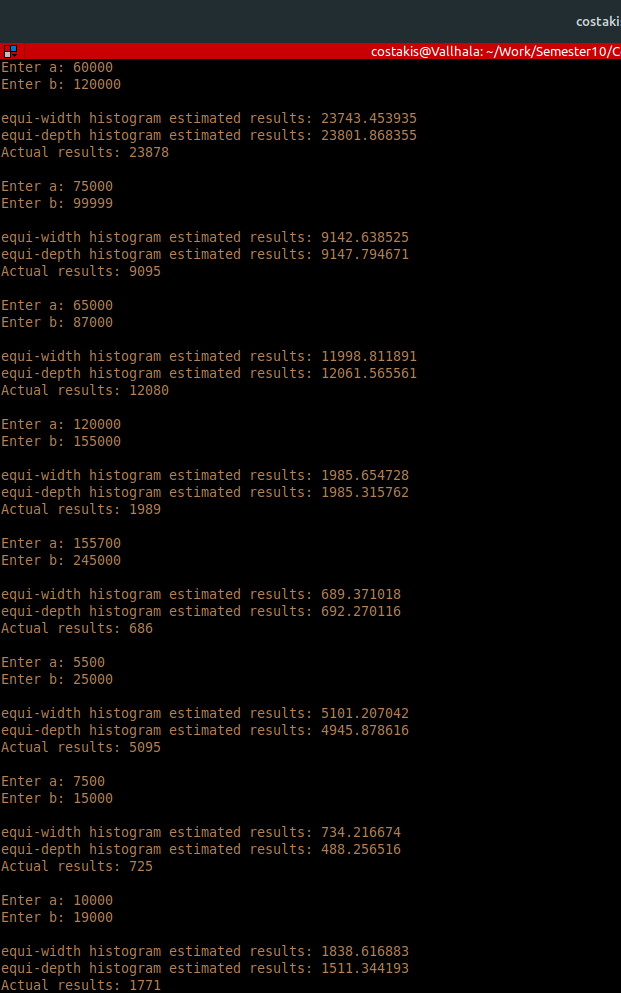
\includegraphics[scale=0.4]{estimations3.png}
\end{figure}
\newpage
Από τα παραπάνω πειράματα είναι αντιληπτό πως το equi-depth histogram υπερτερεί του equi-width histogram για την εκτίμηση των πλειάδεων που έχει το αποτέλεσμα μιας ερώτησης επιλογής στο πεδίο Income, η οποία έχει σαν συνθήκη το $α \leq Income < β.$ Αυτό συμβαίνει καθώς στο equi-depth histogram το κάθε bin έχει ίδιο αριθμό πλειάδων, άρα τα δεδομένα είναι όμοια μοιρασμένα στα ranges του κάθε bin. Στις εικόνες υπάρχουν και περιπτώσεις όπου το equi-width histogram δίνει καλύτερη εκτίμηση και αυτό διότι μπορεί στο συγκεκριμένο εύρος της ερώτησης, το αντίστοιχο bin του ιστογράμματος να μην επικαλύπτεται με κάποιο άλλο, με αποτέλεσμα να είναι πιο ακριβής ο αριθμός των πλειάδων. 
\end{document}